%==============================================================================
% Final poster -- David Quinzanos Saiz
%==============================================================================

\RequirePackage{fix-cm}
\documentclass{article}

\usepackage[
  paperwidth=84.1cm,
  paperheight=118.9cm,
  margin=2.5cm
]{geometry}

\usepackage[utf8]{inputenc}
\usepackage[english]{babel}
\usepackage{amsmath,amssymb}
\usepackage{array}
\usepackage{booktabs}
\usepackage{graphicx}
\usepackage{xcolor}
\usepackage{url}
\usepackage{tikz}
\usetikzlibrary{arrows.meta,positioning,fit,calc,shapes.geometric}
\pagestyle{empty}

\definecolor{posterblue}{RGB}{22,61,102}
\definecolor{posterorange}{RGB}{206,103,37}
\definecolor{postergray}{RGB}{45,45,45}

\setlength{\parindent}{0pt}
\setlength{\parskip}{0.62em}
\renewcommand{\familydefault}{\sfdefault}
\renewcommand{\labelitemi}{\textcolor{posterorange}{\large$\blacktriangleright$}}

\newlength{\postercolwidth}
\setlength{\postercolwidth}{25.05cm}

\newcommand{\highlight}[1]{\textcolor{posterorange}{\textbf{#1}}}
\newcommand{\smalltable}{\fontsize{22}{26}\selectfont}
\newenvironment{posterfigure}
{
  \vspace{0.24cm}
  \begin{center}
}
{
  \end{center}
  \vspace{0.16cm}
}

\newenvironment{posterblock}[1]
{
  \vspace{1.0cm}
  \noindent
  \begin{minipage}{\postercolwidth}
  \colorbox{posterblue}{%
    \parbox{\dimexpr\postercolwidth-2\fboxsep\relax}{%
      \color{white}\bfseries\fontsize{32}{38}\selectfont #1
    }%
  }
  \par\vspace{0.22cm}
  \color{postergray}
  \fontsize{29}{35}\selectfont
}
{
  \end{minipage}
  \par
}

\begin{document}
\fontsize{29}{35}\selectfont

%==============================================================================
% Header
%==============================================================================
\noindent
\colorbox{posterblue}{%
  \begin{minipage}{\dimexpr\textwidth-4\fboxsep\relax}
  \vspace{0.65cm}
  \begin{minipage}{0.13\textwidth}
    \centering
    
\includegraphics[height=4.8cm]{assets/uc.png}
  \end{minipage}%
  \begin{minipage}{0.68\textwidth}
    \centering
    {\color{white}\bfseries\fontsize{46}{54}\selectfont
    Detecting Shared RSA Factors in Certificate Transparency Logs\\
    \fontsize{40}{48}\selectfont a Binary Tree Batch GCD approach\par}
    \vspace{0.45cm}
    {\color{white}\fontsize{29}{35}\selectfont
    David Quinzaños Saiz, Ana I. Gómez Pérez, Domingo Gómez Pérez\par}
    \vspace{0.2cm}
    {\color{white}\fontsize{24}{29}\selectfont
    Department of Mathematics, Statistics and Computing -- University of Cantabria\par}
  \end{minipage}%
  \begin{minipage}{0.13\textwidth}
    \centering
    {\color{white}\fontsize{24}{30}\selectfont
    Final CT-log audit\\
    54,275 RSA moduli\\
    0 vulnerable keys}
  \end{minipage}
  \vspace{0.65cm}
  \end{minipage}
}

%==============================================================================
% Three manual columns
%==============================================================================
\noindent
\begin{minipage}[t]{\postercolwidth}

\begin{posterblock}{Motivation and aim}
RSA security relies on the primes used to build each modulus
$N=p\cdot q$ being unpredictable and never reused. If two moduli share a prime
factor, computing $\gcd(N_i,N_j)$ is enough to compromise both private keys.

This scenario is especially relevant for digital certificates, because the RSA
public key is embedded in the certificate and can be collected openly.
\textit{Certificate Transparency} (CT) logs therefore provide a large public
source of real Internet keys for cryptographic auditing.

Unlike broad Internet scans, CT logs mainly contain certificates accepted by the
public Web PKI and logged for transparency. This makes them a useful empirical
source for studying RSA keys that are actually deployed in the browser-trusted
ecosystem, rather than only in test, internal, or self-signed environments.

The problem was previously studied in the master's thesis \textit{Finding
shared RSA factors in the Certificate Transparency logs}, which analyzes real
certificates extracted from CT logs with classical \textit{batch GCD}
techniques. That work shows the practical value of auditing CT logs, but also
the high computational cost of large-scale analysis.

As an algorithmic improvement, Pelofske proposes \textit{Binary Tree Batch GCD},
a more efficient method that avoids part of the cost of the classical
\textit{remainder tree} approach.

This thesis connects both lines of work: it searches for shared RSA factors in
CT logs, evaluates \textit{Binary Tree Batch GCD} against the classical method,
and develops a C++17/GMP/OpenMP implementation suitable for large-scale runs.
\end{posterblock}

\begin{posterblock}{Algorithm and implementation}
The naive approach requires $\mathcal{O}(M^2)$ GCD computations for $M$ RSA
moduli. Classical \textit{batch GCD} avoids pairwise comparison through a
\textit{product tree} and a \textit{remainder tree}, but the second structure is
expensive in time and memory.

\begin{posterfigure}
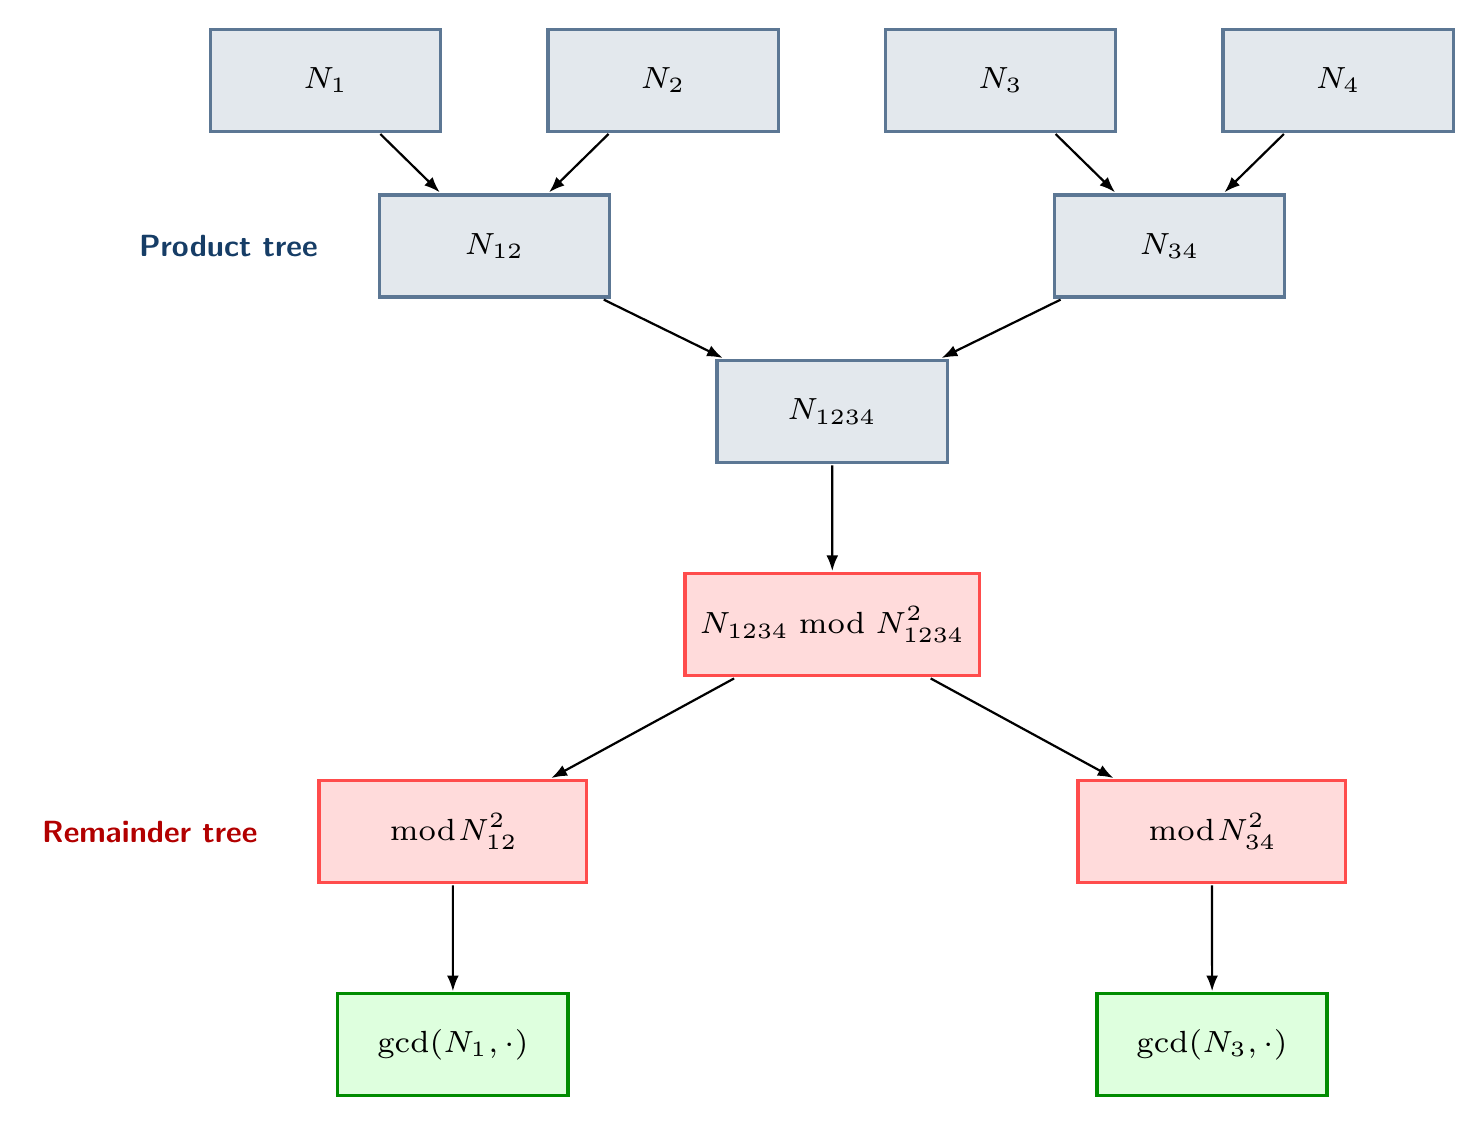
\begin{tikzpicture}[
  scale=1.58,
  transform shape,
  node distance=0.82cm and 0.82cm,
  box/.style={rectangle, draw=posterblue!70, fill=posterblue!12, very thick,
    minimum width=1.85cm, minimum height=0.82cm, font=\scriptsize},
  rem/.style={rectangle, draw=red!70, fill=red!14, very thick,
    minimum width=2.15cm, minimum height=0.82cm, font=\scriptsize},
  gcdnode/.style={rectangle, draw=green!55!black, fill=green!13, very thick,
    minimum width=1.85cm, minimum height=0.82cm, font=\scriptsize},
  arr/.style={-{Latex[length=2mm]}, thick}
]
\node[box] (n1) {$N_1$};
\node[box, right=of n1] (n2) {$N_2$};
\node[box, right=of n2] (n3) {$N_3$};
\node[box, right=of n3] (n4) {$N_4$};
\node[box, below=0.9cm of $(n1)!0.5!(n2)$] (p12) {$N_{12}$};
\node[box, below=0.9cm of $(n3)!0.5!(n4)$] (p34) {$N_{34}$};
\node[box, below=0.9cm of $(p12)!0.5!(p34)$] (pall) {$N_{1234}$};
\node[rem, below=0.85cm of pall] (rall) {$N_{1234}\bmod N_{1234}^2$};
\node[rem, below left=0.8cm and 0.75cm of rall] (r12) {$\bmod N_{12}^2$};
\node[rem, below right=0.8cm and 0.75cm of rall] (r34) {$\bmod N_{34}^2$};
\node[gcdnode, below=0.85cm of r12] (g12) {$\gcd(N_1,\cdot)$};
\node[gcdnode, below=0.85cm of r34] (g34) {$\gcd(N_3,\cdot)$};
\draw[arr] (n1) -- (p12);
\draw[arr] (n2) -- (p12);
\draw[arr] (n3) -- (p34);
\draw[arr] (n4) -- (p34);
\draw[arr] (p12) -- (pall);
\draw[arr] (p34) -- (pall);
\draw[arr] (pall) -- (rall);
\draw[arr] (rall) -- (r12);
\draw[arr] (rall) -- (r34);
\draw[arr] (r12) -- (g12);
\draw[arr] (r34) -- (g34);
\node[font=\scriptsize\bfseries, text=posterblue, left=0.35cm of p12] {Product tree};
\node[font=\scriptsize\bfseries, text=red!70!black, left=0.35cm of r12] {Remainder tree};
\end{tikzpicture}
\end{posterfigure}

\textit{Binary Tree Batch GCD} removes the full \textit{remainder tree}. During
product-tree construction it computes GCDs between sibling branches, stores the
non-trivial GCDs in a single aggregate value $B$, and finally checks
$\gcd(N_i,B)$ for each input modulus. This is efficient when shared factors are
rare compared with the total number of keys, as expected in real CT logs.

\begin{posterfigure}
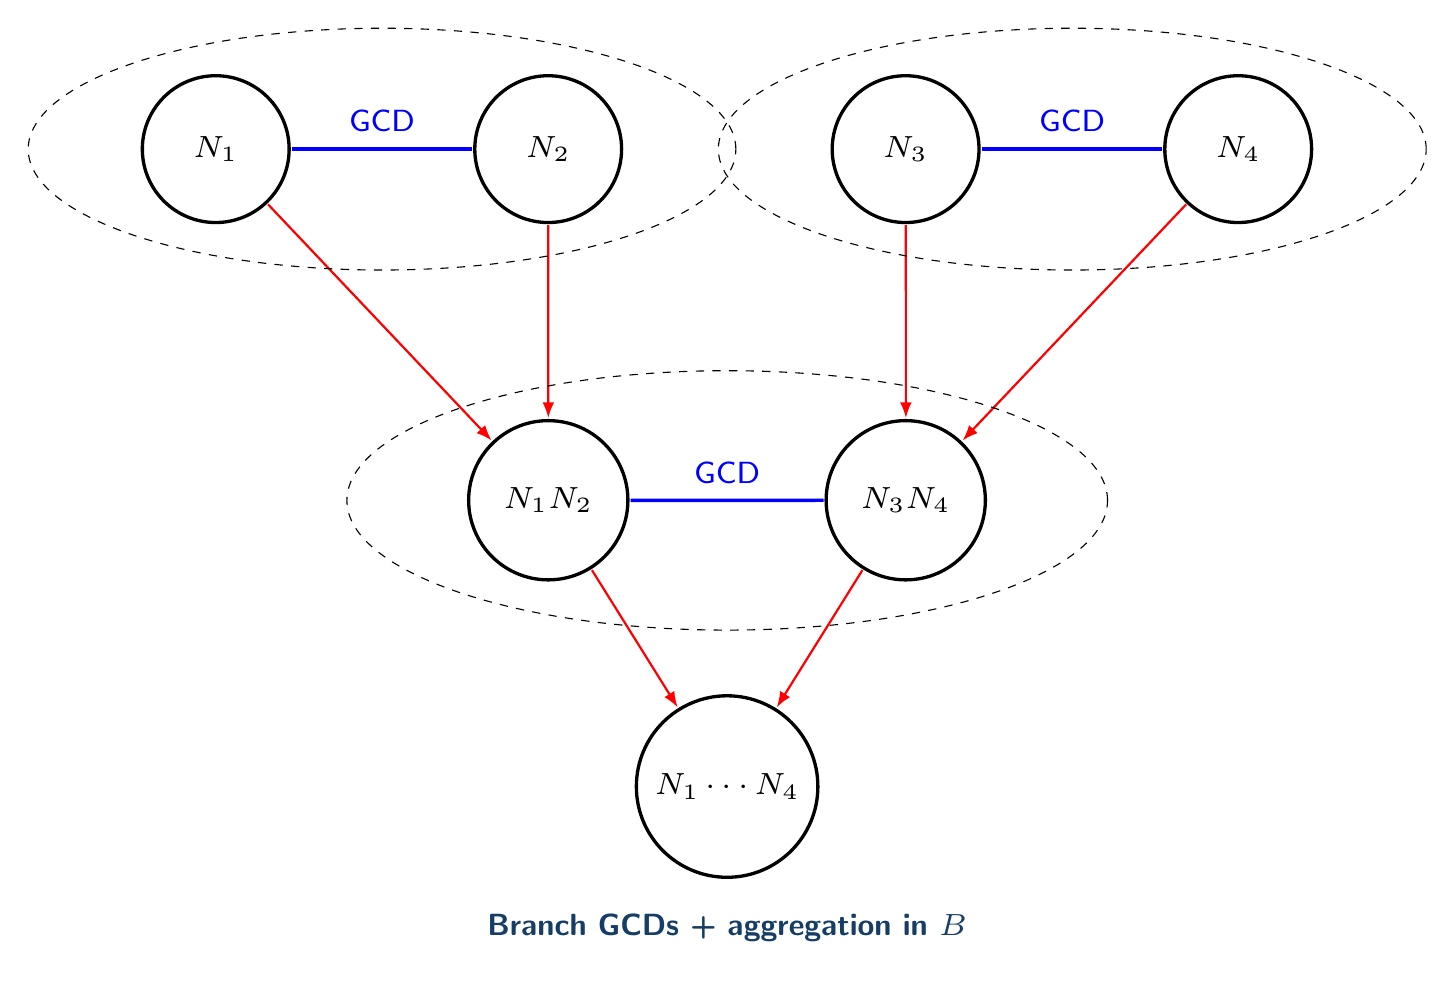
\begin{tikzpicture}[
  scale=1.58,
  transform shape,
  node distance=1.0cm and 0.55cm,
  mod/.style={circle, draw=black, very thick, minimum size=1.18cm, font=\scriptsize},
  prod/.style={circle, draw=black, very thick, minimum size=1.28cm, font=\scriptsize},
  group/.style={ellipse, draw=black, dashed, inner xsep=0.1cm, inner ysep=0.12cm},
  gcd/.style={blue, very thick},
  edge/.style={red, thick, -{Latex[length=2mm]}}
]

\node[mod] (bn1) {$N_1$};
\node[mod, right=1.45cm of bn1] (bn2) {$N_2$};
\node[mod, right=1.65cm of bn2] (bn3) {$N_3$};
\node[mod, right=1.45cm of bn3] (bn4) {$N_4$};

\node[prod, below=1.55cm of bn2] (bp12) {$N_1N_2$};
\node[prod, below=1.55cm of bn3] (bp34) {$N_3N_4$};
\node[prod, below=1.55cm of $(bp12)!0.5!(bp34)$] (bpall) {$N_1\cdots N_4$};

\draw[gcd] (bn1) -- node[above, font=\scriptsize] {GCD} (bn2);
\draw[gcd] (bn3) -- node[above, font=\scriptsize] {GCD} (bn4);
\draw[gcd] (bp12) -- node[above, font=\scriptsize] {GCD} (bp34);

\draw[edge] (bn1) -- (bp12);
\draw[edge] (bn2) -- (bp12);
\draw[edge] (bn3) -- (bp34);
\draw[edge] (bn4) -- (bp34);
\draw[edge] (bp12) -- (bpall);
\draw[edge] (bp34) -- (bpall);

\node[group, fit=(bn1)(bn2)] {};
\node[group, fit=(bn3)(bn4)] {};
\node[group, fit=(bp12)(bp34)] {};
\node[font=\scriptsize\bfseries, text=posterblue, below=0.15cm of bpall]
{Branch GCDs + aggregation in $B$};
\end{tikzpicture}
\end{posterfigure}

The implementation follows three phases: product-tree construction with
in-line GCD computation, aggregation of non-trivial GCDs into $B$, and final
enumeration of the original moduli through $\gcd(N_i,B)$. Intermediate products
are released as soon as they are no longer needed, and the final enumeration is
parallelized with OpenMP.

Pelofske's Python versions are used as references, but Python overhead on large
integers limits scalability. The final implementation therefore uses C++17 with
GMP and OpenMP to improve multiprecision arithmetic, memory control, and
parallel enumeration.
\end{posterblock}

\end{minipage}
\hfill
\begin{minipage}[t]{\postercolwidth}

\begin{posterblock}{Experimental design}
Validation combines two phases. First, synthetic experiments use RSA moduli of
1024 and 2048 bits with a controlled number of weak keys. This checks that the
algorithm detects the inserted shared factors and measures execution time as the
input size grows.

\begin{posterfigure}
\makebox[\postercolwidth][c]{%
  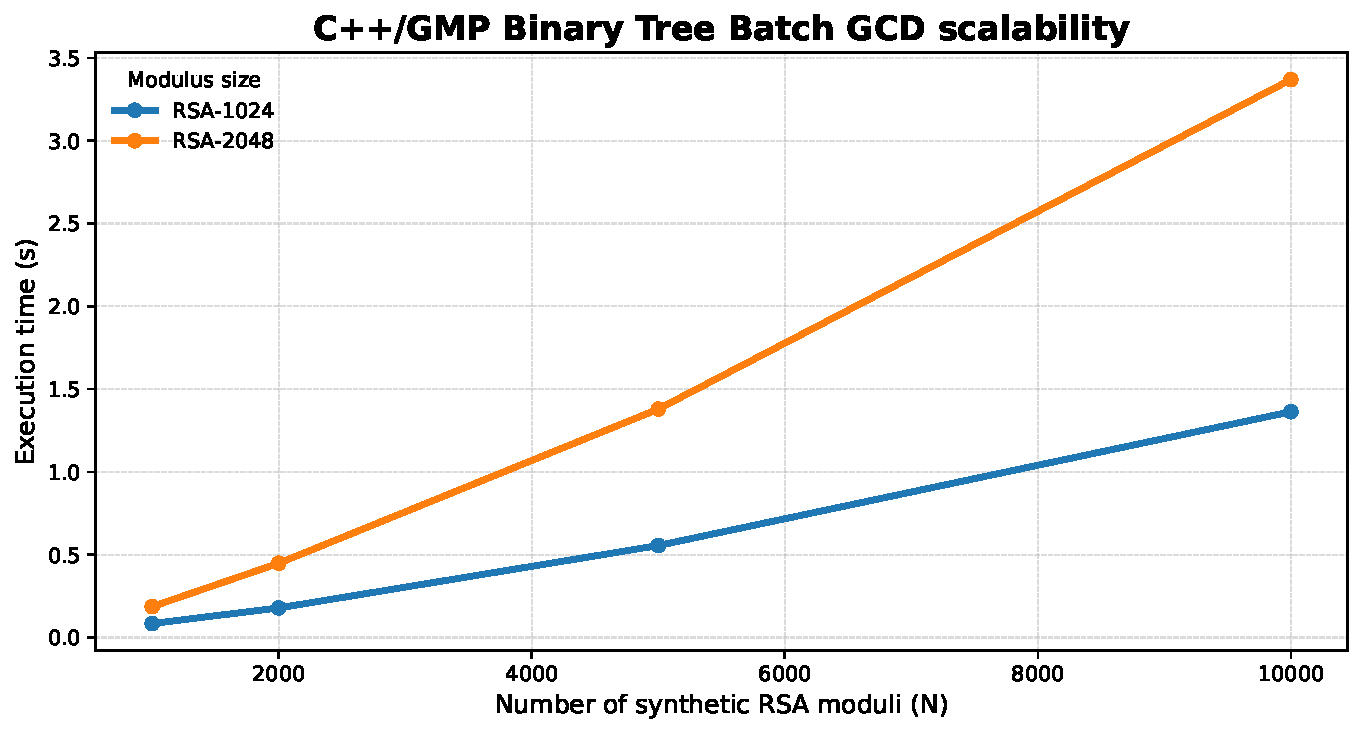
\includegraphics[width=1.02\postercolwidth]{assets/scalability_batch_gcd_en.pdf}%
}
\end{posterfigure}

Second, the repository associated with Pelofske's article is used to reproduce a
comparison close to the original experiment. The benchmark evaluates three
variants on the same inputs: classical \textit{Remainder Tree Batch GCD} in
Python, \textit{Binary Tree Batch GCD} in Python, and the C++/GMP implementation
developed in this thesis.

For each configuration, synthetic RSA moduli are written as hexadecimal values,
one modulus per line. The same input file is then used by all three algorithms,
so the comparison reflects the algorithmic and implementation cost rather than
differences in the generated data.

Integrating the reference repository required adapting the code to current
Python and NumPy versions, adding execution wrappers, normalizing module input,
and generating the additional primes required for RSA-2048 tests.
\end{posterblock}

\begin{posterblock}{Benchmark results}
\begin{posterfigure}
\makebox[\postercolwidth][c]{%
  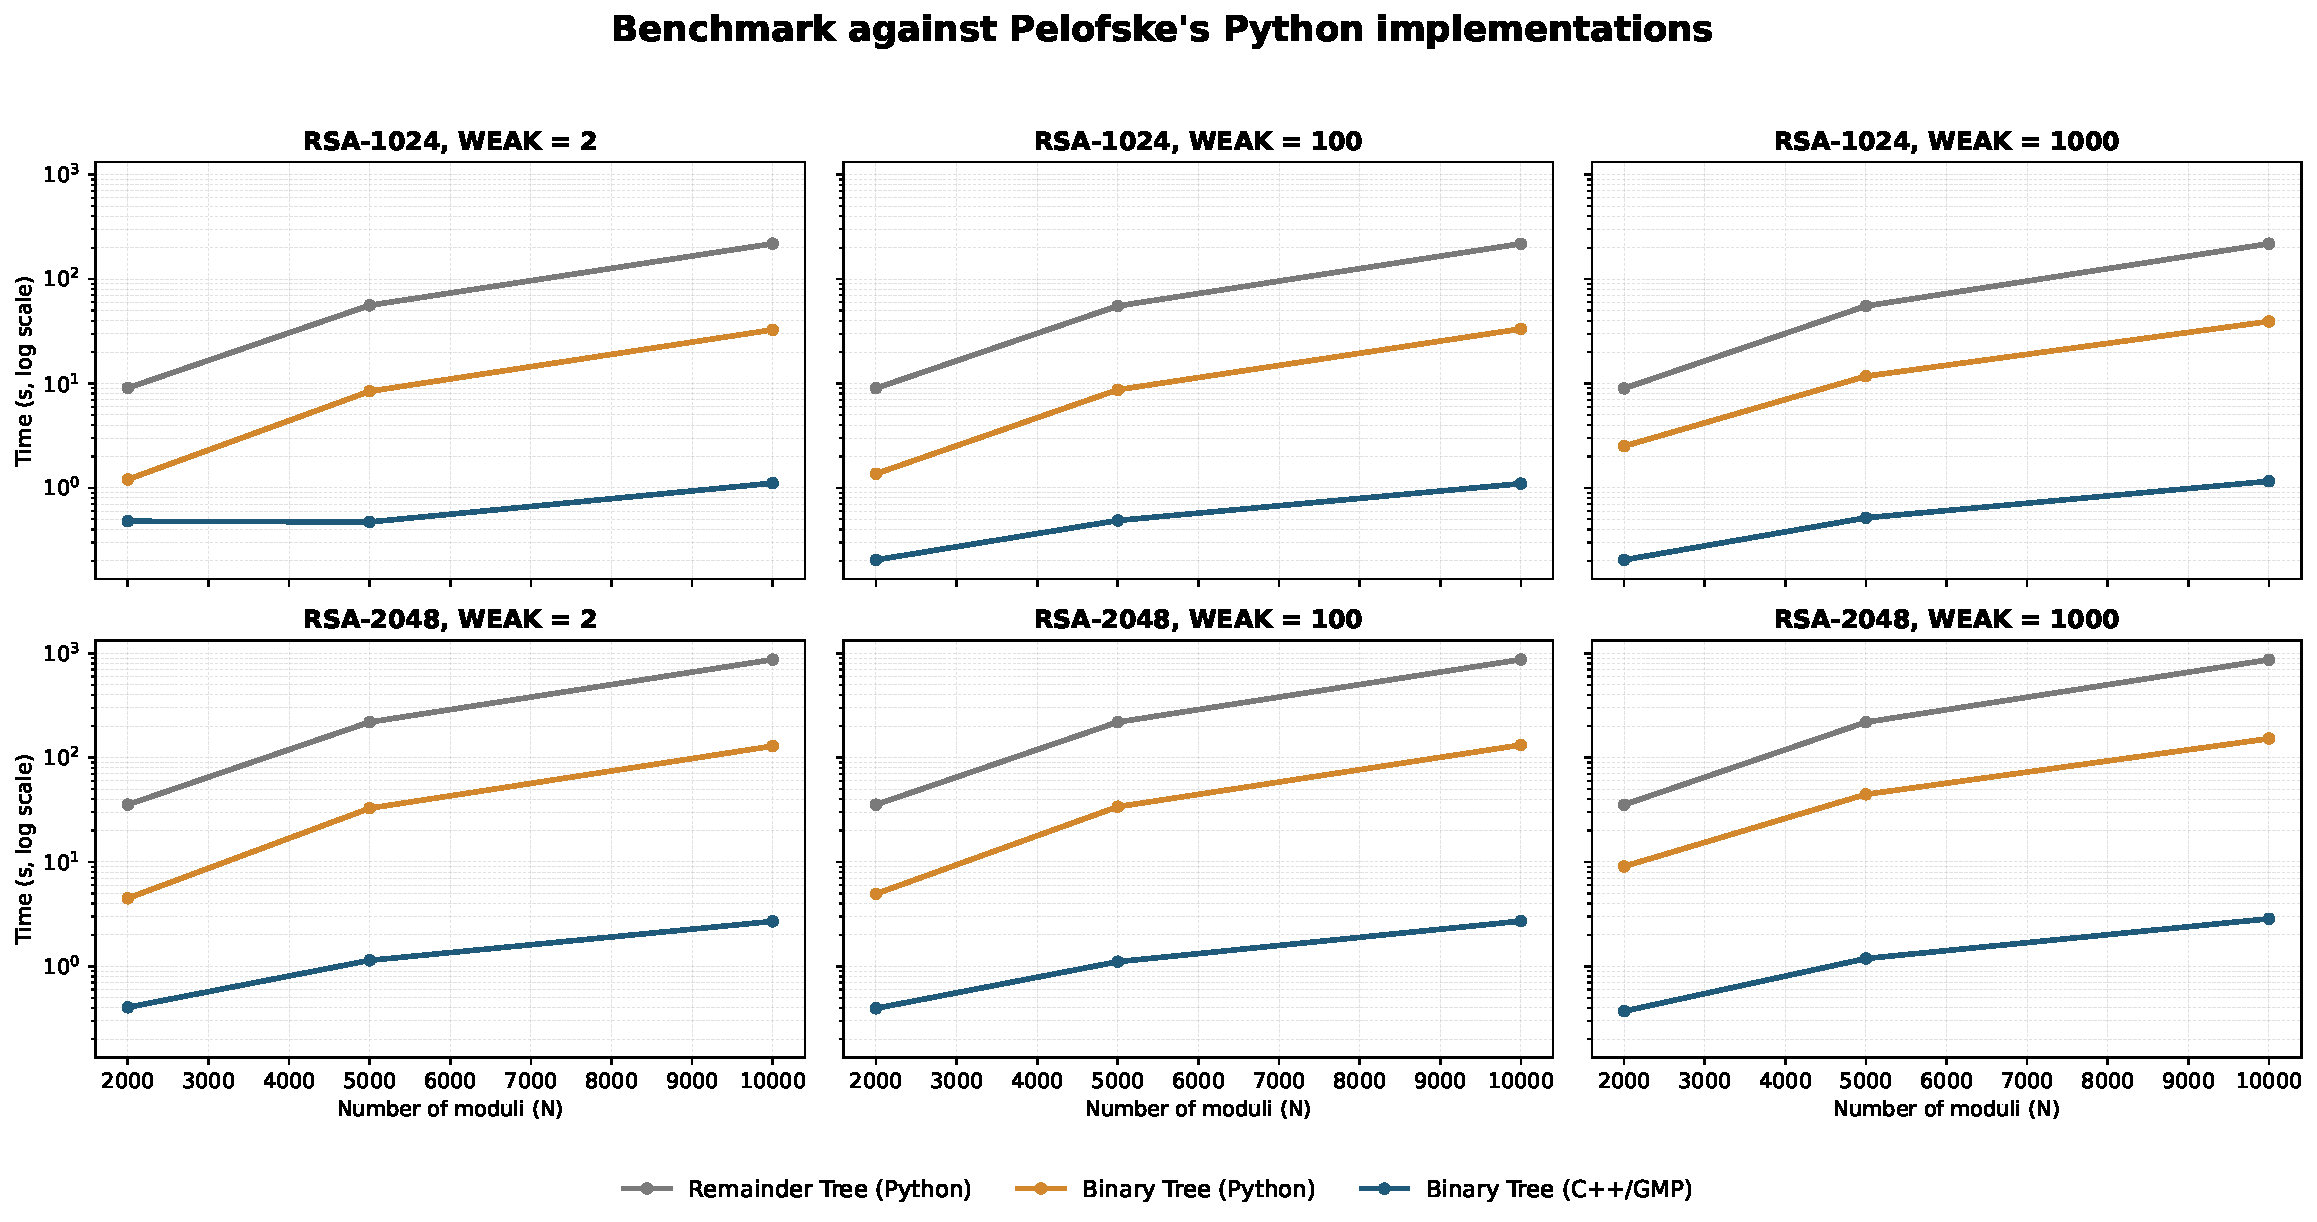
\includegraphics[width=1.02\postercolwidth]{assets/pelofske_time_en.pdf}%
}
\end{posterfigure}

The extended benchmark contains 18 completed configurations combining 1024- and
2048-bit RSA moduli, three input sizes, and three values of \texttt{WEAK}. Across
those configurations, Python \textit{Binary Tree Batch GCD} is on average
$6.1\times$ faster than Python \textit{Remainder Tree Batch GCD}. The C++/GMP
implementation is on average $156.9\times$ faster than Python
\textit{Remainder Tree Batch GCD} and $26.0\times$ faster than Python
\textit{Binary Tree Batch GCD}.

The vertical axis is logarithmic because the runtime gap between Python and
C++/GMP is too large for a linear comparison. The same synthetic input was used
by the three implementations and the detected vulnerable moduli matched, so the
figure compares execution cost rather than differences in correctness. The
pattern is consistent: increasing $N$ dominates runtime, RSA-2048 is slower than
RSA-1024, and avoiding the explicit \textit{remainder tree} is always beneficial.
\end{posterblock}

\begin{posterblock}{Observed speed-up}
The most demanding local benchmark configuration uses RSA-2048 moduli,
$N=10000$ and \texttt{WEAK}=1000: the classical Python method takes 867.508 s,
Pelofske's Python binary-tree version takes 152.171 s, and the C++/GMP
implementation takes 2.860 s.

\vspace{0.25cm}
{\smalltable
\begin{center}
\begin{tabular}{cccrrr}
\toprule
Bits & \texttt{WEAK} & $N$ & Remainder Py. & Binary Py. & Binary C++ \\
\midrule
1024 & 100  & 10000 & 218.468 s & 33.337 s  & 1.097 s \\
2048 & 100  & 10000 & 870.560 s & 132.189 s & 2.714 s \\
2048 & 1000 & 10000 & 867.508 s & 152.171 s & 2.860 s \\
\bottomrule
\end{tabular}
\end{center}
}

\vspace{0.2cm}
{\centering
  \colorbox{posterorange}{%
    \parbox{0.86\postercolwidth}{%
      \centering\color{white}\bfseries
      C++/GMP reaches up to $322.4\times$ speed-up over the classical Python method.
    }%
  }\par
}

\vspace{0.12cm}
In practical terms, the hardest displayed case moves from more than 14 minutes
with the classical Python baseline to under 3 seconds with the C++/GMP binary.
That margin makes repeated validation, archive corrections, and real-data reruns
feasible within the same CT-log audit workflow.
\end{posterblock}

\end{minipage}
\hfill
\begin{minipage}[t]{\postercolwidth}

\begin{posterblock}{Real RSA Modulus Extraction}
The real-data pipeline starts from selected public \texttt{ct-archive} ZIP
files. The workflow is incremental: one archive is downloaded, inspected and
processed independently, then only the extracted metadata needed for the audit
is kept. This avoids storing full certificate collections permanently and makes
large or problematic ZIP files easier to retry. The extraction state of each
ZIP is tracked explicitly so interrupted downloads, Zip64 issues, and archives
without \texttt{issuer/} entries can be treated conservatively.

Only X.509 issuer certificates under the \texttt{issuer/} directory are parsed.
OpenSSL extracts both the RSA public-key modulus and the certificate issuer.
The intermediate output keeps pairs of the form \texttt{modulus||issuer}; the
issuer is not needed for Batch GCD, but it would provide context if a vulnerable
modulus were found.

\begin{posterfigure}
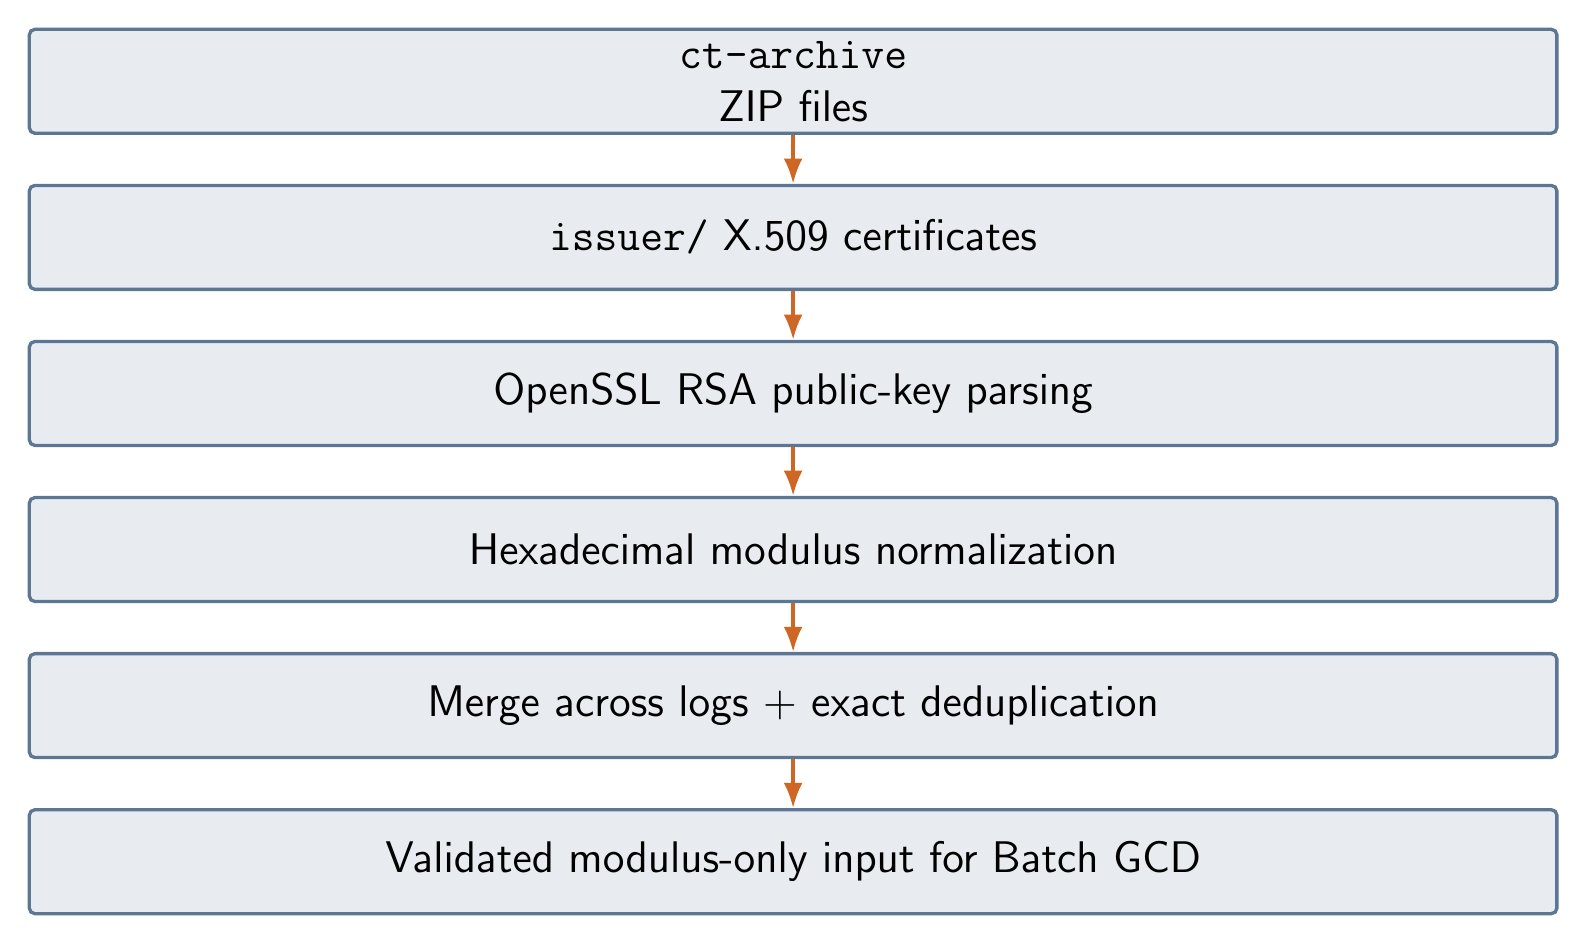
\begin{tikzpicture}[
  node distance=0.62cm,
  stage/.style={rectangle, rounded corners=2pt, draw=posterblue!70,
    fill=posterblue!10, very thick, align=center,
    minimum width=19.4cm, minimum height=1.32cm,
    font=\fontsize{16}{19}\selectfont},
  arrow/.style={-{Latex[length=3.2mm]}, line width=1.2pt, draw=posterorange}
]
\node[stage] (zips) {\texttt{ct-archive}\\ZIP files};
\node[stage, below=of zips] (issuer) {\texttt{issuer/} X.509 certificates};
\node[stage, below=of issuer] (parse) {OpenSSL RSA public-key parsing};
\node[stage, below=of parse] (hex) {Hexadecimal modulus normalization};
\node[stage, below=of hex] (dedup) {Merge across logs + exact deduplication};
\node[stage, below=of dedup] (input) {Validated modulus-only input for Batch GCD};

\draw[arrow] (zips) -- (issuer);
\draw[arrow] (issuer) -- (parse);
\draw[arrow] (parse) -- (hex);
\draw[arrow] (hex) -- (dedup);
\draw[arrow] (dedup) -- (input);
\end{tikzpicture}
\end{posterfigure}

\begin{itemize}
  \item Processing \texttt{issuer/} avoids traversing the full CT tile data and
  keeps the extraction feasible ZIP by ZIP.
  \item Each archive is recorded as processed, failed, or apparently without
  \texttt{issuer/}; suspicious cases are reviewed before being discarded.
  \item The \texttt{Modulus=} prefix and formatting artifacts are removed, so
  each output line contains exactly one hexadecimal integer.
  \item Duplicates caused by renewals, equivalent certificates, or repeated
  appearances across logs are removed before the GCD computation.
  \item Plausibility validation checks the modulus-only input before the
  C++/GMP binary runs.
\end{itemize}
\end{posterblock}

\begin{posterblock}{Final CT-Log Audit}
The final audit uses this clean modulus-only input after normalization, exact
deduplication, and validation of plausible RSA moduli. The validation step
removes malformed values and checks that the remaining integers behave like RSA
moduli suitable for the attack input.

{\smalltable
\begin{center}
\begin{tabular}{@{}p{16.2cm}r@{}}
\toprule
Metric & Value \\
\midrule
Raw unique RSA moduli & 54,278 \\
Plausible RSA moduli analyzed & 54,275 \\
Moduli discarded during validation & 3 \\
CT logs with extracted moduli & 20 \\
Incomplete logs at execution time & 0 \\
Non-trivial GCDs in phase 1 & 0 \\
Vulnerable keys detected & 0 \\
Total algorithm time & 23.756 s \\
\bottomrule
\end{tabular}
\end{center}
}

The final run did not detect shared RSA factors in the analyzed data set. This
does not prove that all CT-log certificates are safe; it states that no shared
factor was found in the final deduplicated set processed by this thesis. The
result is therefore an applied audit result for this extracted data set, not a
global claim about every certificate ever logged in CT.
\end{posterblock}

\begin{posterblock}{Conclusions}
\begin{itemize}
  \item \textit{Binary Tree Batch GCD} reduces the practical cost of shared
  factor detection compared with the classical \textit{remainder tree} method.
  \item The C++17/GMP implementation clearly outperforms the original Python
  implementations on the reproduced benchmark.
  \item The complete extraction, normalization, validation, and analysis flow
  was run on real CT-log data.
  \item No vulnerable RSA key was detected among the 54,275 plausible unique RSA
  moduli analyzed.
\end{itemize}

The main contribution is a reproducible end-to-end workflow that links CT-log
data engineering with an efficient shared-factor audit for real RSA public
keys.
\end{posterblock}

\begin{posterblock}{References}
\fontsize{18}{22}\selectfont
R. L. Rivest, A. Shamir, L. Adleman, ``A method for obtaining digital signatures and public-key cryptosystems'', \textit{Communications of the ACM}, 1978.

N. Heninger et al., ``Mining Your Ps and Qs'', \textit{USENIX Security}, 2012.

H. F. Våge, ``Finding shared RSA factors in the Certificate Transparency logs'', Master's Thesis, University of Bergen, 2022.

E. Pelofske, ``An Efficient All-to-All GCD Algorithm for Low Entropy RSA Key Factorization'', Preprint, 2024.
\end{posterblock}

\end{minipage}

\end{document}
